Når en ladet kondensator står i en lukket krets med motstand,
vil kondensatoren lade seg ut.
\\\\
\begin{circuitikz} \draw
(0,0) to[C, label=$C$] (0,2)
      -- (4,2)
      to[R, label=$R$] (4,0)
      -- (0,0)
      ;
\end{circuitikz}
\\\\
Spenningen U  er gitt ved $U = R \cdot I$.
\\
Spenningen til kondensatoren kaller vi V.
\\
Etter kirchhoffs lov om spenninger er
summen av alle spenninger i en krets lik null.
\\
$$R \cdot I + V = 0$$
\\\\
Strøm I er gitt ved
$$I = C \cdot \frac{dV}{dt}$$
\\\\
Satt inn for I gir det
$$R \cdot C \cdot \frac{dV}{dt} + V = 0$$
\\\\
Løser man dette for spenningen over kondensatoren får man
$$V_C(t) = V_0 \cdot e^{\frac{-t}{RC}} = V_0 \cdot e^{\frac{-t}{\tau}}$$
Hvor $\tau = RC$ er \emph{tidskonstanten}.
\\\\
Etter en tid $\tau$ har størrelsen blitt redusert
til ca 37\% av startverdien.
Etter $5 \tau$ er størrelsen redusert til 1\%
og kondensatoren anses som utladet.
\\
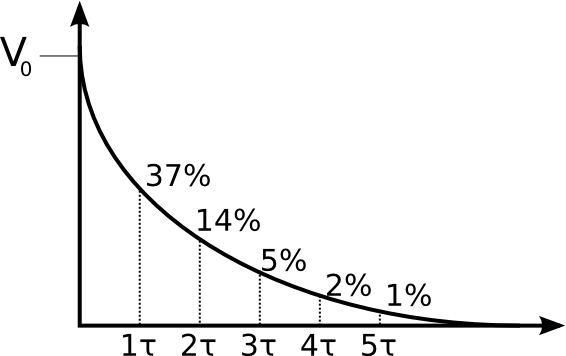
\includegraphics[width=0.5\textwidth]{./img/tidskonstant}
